\documentclass[12pt]{article}
\usepackage[a4paper, margin=.30in]{geometry}
\usepackage{graphicx ,
            wrapfig,
            xcolor, 
            enumerate,
            amsmath,fontenc, mhchem,makecell, mhchem,tcolorbox
            }

\newcommand\headerMe[2]{\noindent{}#1\hfill#2}
\renewcommand{\thesection}{\Roman{section}}

\author{Zakaria HAOUZAN}
\date{\today}

\begin{document}
% headers --------------
\headerMe{Matière : Physique-Chimie}{Professeur : Zakaria HAOUZAN}\\
\headerMe{Unité : Transformations non totales d'un\\système chimique  }{Établissement : Lycée SKHOR qualifiant}\\
\headerMe{Niveau : 2BAC-SM-PC}{Heure : 4H}\\

% ------Content ________
\begin{center}

    \Large{Leçon $N^{\circ} 3.2 $: \color{red} Etat d'équilibre d'un système chimique }
\end{center}

\section{Quotient de la réaction :}
\subsection{Définition :}
Le quotient de la réaction est une grandeur qui caractérise un système chimique dans un état donné.

Sa valeur nous renseigne sur l'évolution du système étudié.
On considère la transformation chimique modélisée par la réaction suivante:

$$\ce{\alpha.A_{(aq)} + \beta.B_{(aq)} <=> \gamma.C_{(aq)} + \delta.D_{(aq)}}$$
Le quotient de cette réaction  s'écrit : $$Q_r = \frac{[C]^{\gamma}.[D]^{\delta}}{[A]^{\alpha}.[B]^{\beta}}$$

$Q_r$ est une grandeur sans Unité.

[A],[B],[C] et [D] concentrations molaires des espéces chimiques exprimées en mol/L.

\subsection{Convetion : }
Par convention dans l'expression de Qr, il ne figure que les concentrations.molaires.des.espèces.dissoutes (le solvant "eau" ou les solides n'interviennent pas).
\subsection{Exemples : }
\begin{itemize}
	\item \underline{Réaction dans tous les réactifs et les produits sont à l'état aqueux :}

$\ce{{I_2}_{(aq)} + 2{S_2O_3^{2-}}_{(aq)} <=>[1][2] 2I^-_{(aq)} + S_4O_6^{2-}_{(aq)}}$
\hspace{4cm} $Q_r = \frac{[I^-]^2.[S_4O_6^{2-}]}{[I_2].[S_2O_3^{2-}]^2}$

\item \underline{Réaction dans laquelle le solvant "eau" intervient comme réactif:}

$\ce{CH_3COOH_{(aq)} + H_2O_{(l)} <=>[1][2] CH_3COOH^-_{(aq)}  + H_3O^+_{(aq)} }$
\hspace{2cm} $Q_r = \frac{[CH_3COO^-].[H_3O^+]}{[CH_3COOH]}$

\item \underline{Réaction dans laquelle interviennent les solides: }

	$\ce{Cu_{(s)} + 2Ag^+_{(aq)} <=>[1][2] Cu^{2+}_{(aq)} + 2Ag_{(s)}}$
	\hspace{5cm} $Q_r = \frac{[Cu^{2+}]}{[Ag^+]^2}$

$\ce{Fe^{2+}_{(aq)} + 3OH^-_{(aq)} <=>[1][2] {Fe(OH)_3}_{(s)}}$
\hspace{5cm} $Q_r = \frac{1}{[Fe^{3+}][OH^-]^3}$
\end{itemize}
\section{Le quotient de réaction à l'état d'équilibre : }

\subsection{Définition : }
Le quotient de réaction à l'état d'équilibre (noté Qr, éq) est la valeur que prend le quotient de réaction lorsque l'état d'équilibre du système chimique est atteint.

A l'état d'équilibre, les concentrations des espèces en solution ne varient plus. Elles peuvent être déterminées par des
méthodes chimiques ou physiques comme le dosages, la pH-métrie ou la conductimétrie.

\subsection{Exemple: Réaction de l'acide éthanoïque avec l'eau: }
En mesurant la conductivité d'une solution d'acide éthanoïque de concentration           $C=5.10^{-2}mol/L$ , on trouve $\sigma = 343\mu.S/cm$.

1. Déterminer les concentrations molaire des espèces chimiques dissoutes dans la solution à l'équilibre.

2. Déterminer la valeur du quotient de la réaction à l'équilibre Qr, éq.

On donne : $\lambda_{(CH_3COO^-)} = 4,09mS.m^2/mol$ ; $\lambda_{(H_3O^+)} = 35mS.m^2/mol$

\section{La constante d'équilibre K associée à une  transformation chimique : }
\subsection{Quotient de la réaction à équilibre et à température constante:}
Les études expérimentales ont montrées que le quotient de la réaction à l'équilibre à la même température
reste constant quel soit l'état initial du système .

\subsection{Définition de la constante d'équilibre : }
La constante d'équilibre K associée à l'équation d'une réaction est la valeur que prend le quotient de réaction
Qr, éq. à l'état d'équilibre du système.


$$\ce{\alpha.A_{(aq)} + \beta.B_{(aq)} <=> \gamma.C_{(aq)} + \delta.D_{(aq)}}$$
Le quotient de cette réaction  s'écrit : $$K =Q_{r,eq} = \frac{[C]^{\gamma}.[D]^{\delta}}{[A]^{\alpha}.[B]^{\beta}}$$



\begin{tcolorbox}
	Remarque:
La constante d'équilibre est associée à l'équation d'une réaction écrite dans un sens donné, si l'on
écrit l'équation dans l'autre sens , sa constante d'équilibre sera l'inverse de la précédente.


$$\ce{\alpha.A_{(aq)} + \beta.B_{(aq)} <=> \gamma.C_{(aq)} + \delta.D_{(aq)}}$$
Le quotient de cette réaction  s'écrit : $$K' = \frac{1}{K} = \frac{[C]^{\gamma}.[D]^{\delta}}{[A]^{\alpha}.[B]^{\beta}}$$


La transformation limitée conduit à un état d’équilibre donc l'état final correspond à l’état d'équilibre $x_f = x_{eq}$

\end{tcolorbox}


\section{Influence de l'état initial et de La constante d'équilibre sur le taux d'avancement à  l'équilibre: }
\subsection{Influence de l'état initial:}
Considérons le cas de la réaction de l'acide éthanoïque avec l'eau: 

\begin{tabular}{|c|c|c|c|c|c|}
    \hline
    \multicolumn{2}{|c|}{Equation de la réaction}& \multicolumn{4}{c|}{
\ce{CH_3COOH + H_2O <=>[1][2] CH_3COO^- + H_3O^+}}\\\hline
    états  & avancement& \multicolumn{4}{|c|}{quantité de Matière en mol}\\\hline
	Etat initial          &    0        &  $n_i$ &  - &  0              &  0 \\\hline
                 \makecell{Etat de \\transformation}&    $x$      & $n_i -x$ & - & $x$  & $x$ \\\hline
				 Etat final            & $x_{eq}$ & $n_i - x_{eq}$ & -  & $x_{eq}$&$x_{eq}$ \\\hline
   % \cline{2-4}\
\end{tabular}

L'eau est utilisée en excès ,donc $CH_3COOH$ est le réactif limitant : 
$$x_{max} = C.V$$ et $$x_f = [H_3O^+]_{eq}.V = 10^{-pH}.V$$

Le taux d'avancement de la réaction $$\tau = \frac{x_{eq}}{x_{max}} = \frac{10^{-pH}.V}{CV} = \frac{10^{-pH}}{C}$$

Donc le taux d'avancement de la réaction dépend de l'état initial du système.

Plus la solution d'acide est diluée, plus le taux d'avancement à l'équilibre est grand.

\subsection{Influence de La constante d'équilibre:}

Considérons comme exemple simple la réaction d'équation : 
$$\ce{\alpha.A_{(aq)} + \beta.B_{(aq)} <=> \gamma.C_{(aq)} + \delta.D_{(aq)}}$$

Dans lequel les réactifs ont même concentration initial : C

la constante d’équilibre dans ce cas : $$K = \frac{[C][D]}{[A][B]}$$







Or les deux réactifs sont limitants: $$x_{max} = C.V$$ et $$\tau = \frac{x_{eq}}{CV}$$

$$[A] = [B] = \frac{CV-x_{eq}}{V} = \frac{CV-\tau.CV}{V} = C-\tau.C = C(1-\tau)$$
$$[C] = [D] = \frac{x_{eq}}{V} = \frac{\tau.C.V}{V} = \tau.C$$


Cette expression montre que le taux d'avancement de la réaction dépend de la constante d'équilibre K.

Plus que la constante d'équilibre K est grande plus que le taux d'avncement de la réaction est élevé.

la constante d’équilibre : $$K = \frac{[C].[D]}{[A].[B]} = \frac{\tau^2}{(1-\tau)^2}$$

avec $0 \leq \tau \leq 1$ 


si $K>10^4$ la réaction est considérée comme totale.


%\begin{figure}[h!]
	%\begin{center}
	%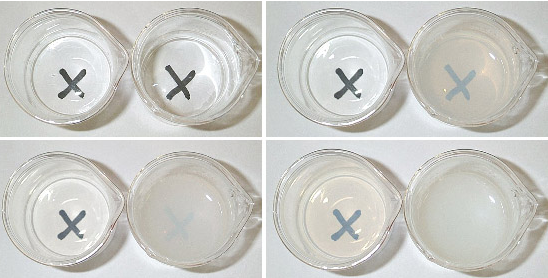
\includegraphics[width=0.5\textwidth]{./img/TRLconcentration.png}
%\end{center}
%\vspace{-1cm}
%\end{figure}



%\begin{wrapfigure}[10]{r}{0.5\textwidth}
%    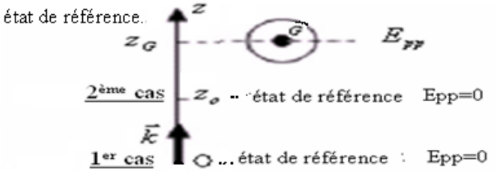
\includegraphics[width=0.5\textwidth]{./img/img00.png}
%\end{wrapfigure}


%\begin{center}
   %\begin{tabular}{|c|c|c|}
      %\hline
      %Indicateur coloré & Couleur de l’espèce acide & Couleur de l’espèce base\\\hline
      %BBT               & Jaune                     & Bleue\\\hline
      %Hélianthine       &Rose                       & Jaune\\\hline
      %Phénolphtaléine   & inclore                   & rose \\\hline
   %\end{tabular}
%\end{center}

\end{document}

